%%%%%%%%%%%%%%%%%%%%%%%%%%%%%%%%%%%%%%%%%
% Beamer Presentation
% LaTeX Template
% Version 1.0 (10/11/12)
%
% This template has been downloaded from:
% http://www.LaTeXTemplates.com
%
% License:
% CC BY-NC-SA 3.0 (http://creativecommons.org/licenses/by-nc-sa/3.0/)
%
%%%%%%%%%%%%%%%%%%%%%%%%%%%%%%%%%%%%%%%%%

%----------------------------------------------------------------------------------------
%	PACKAGES AND THEMES
%----------------------------------------------------------------------------------------

\documentclass{beamer}

\mode<presentation> {

\usetheme{Madrid}
\usecolortheme{dolphin}
%\setbeamertemplate{footline} % To remove the footer line in all slides uncomment this line
%\setbeamertemplate{footline}[page number] % To replace the footer line in all slides with a simple slide count uncomment this line

%\setbeamertemplate{navigation symbols}{} % To remove the navigation symbols from the bottom of all slides uncomment this line
}

\usepackage{graphicx} % Allows including images
\usepackage{ragged2e} % Jusitfy
\usepackage{booktabs} % Allows the use of \toprule, \midrule and \bottomrule in tables
\usepackage{lmodern}
\usepackage{amsfonts}
\usepackage{amsmath}
\usepackage{mathtools}
\usepackage{multicol}
\usepackage{listings} % C++ code
\lstset{language=C++,
                basicstyle=\footnotesize\ttfamily,
                keywordstyle=\footnotesize\color{blue}\ttfamily,
}
\addtobeamertemplate{block begin}{}{\justifying} %Justify
%----------------------------------------------------------------------------------------
%	TITLE PAGE
%----------------------------------------------------------------------------------------

\title[Queues]{Queues} % The short title appears at the bottom of every slide, the full title is only on the title page

\author{Ulises M\'endez Mart\'{i}nez} % Your name
\institute[UTM] % Your institution as it will appear on the bottom of every slide, may be shorthand to save space
{
Algorist Weekly Talks \\ % Your institution for the title page
\medskip
\textit{ulisesmdzmtz@gmail.com} % Your email address
}
\date{\today} % Date, can be changed to a custom date

\begin{document}

\begin{frame}
\titlepage % Print the title page as the first slide
\end{frame}


%--------------------------------------------------------
%-- OVERVIEW SECTION
%--------------------------------------------------------
\begin{frame}
\frametitle{Overview} % Table of contents slide, comment this block out to remove it
\tableofcontents % Throughout your presentation, if you choose to use 
\end{frame}
%--------------------------------------------------------
%	PRESENTATION SLIDES
%--------------------------------------------------------

%--------------------------------------------------------
\section{Queues} 
\subsection{Introduction}
\begin{frame}
\frametitle{ FIFO or LILO?}
\begin{figure}
	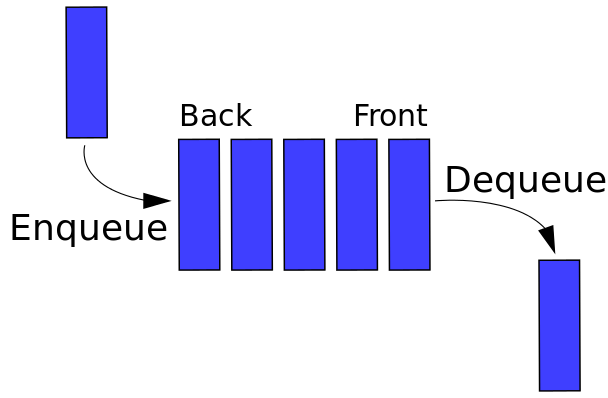
\includegraphics[width=0.7\linewidth]{queue.png}
	\caption{Representation of a FIFO (first in, first out) queue}
\end{figure}
\end{frame}

\begin{frame}
\frametitle{ FIFO }
In a FIFO data structure, the first element added to the queue will be the first one to be removed. This is equivalent to the requirement that once a new element is added, all elements that were added before have to be removed before the new element can be removed.
\end{frame} 
%--------------------------------------------------------

\subsection{C++ STL Queue} 

\begin{frame}
\frametitle{C++ STL Queue}

\begin{block}{std::queue}
template $<$class T, class Container = deque$<$T$>$ $>$ class queue;
\end{block}

\textbf{FIFO queue}\\
queues are a type of container adaptor, specifically designed to operate in a FIFO context (first-in first-out), where elements are inserted into one end of the container and extracted from the other.

\begin{multicols}{2}
\begin{itemize}
	\item empty
	\item size
	\item front
	\item back
	\item push\_back
	\item pop\_front
\end{itemize}
\end{multicols}

The standard container classes deque and list fulfill these requirements. By default, if no container class is specified for a particular queue class instantiation, the standard container deque is used.

\end{frame}
%--------------------------------------------------------
\subsection{Challenge (Easy)}
\begin{frame}
\frametitle{Throwing cards away I (Easy)}

\begin{block}{Description}
Given is an ordered deck of $n$ cards numbered $1$ to $n$ with card $1$ at the top and card $n$ at the bottom. The following operation is performed as long as there are at least two cards in the deck:\\
Throw away the top card and move the card that is now on the top of the deck to the bottom of the deck.\\
\textbf{Your task is to  find the sequence of discarded
cards and the last, remaining card.}
\end{block}

\end{frame}
%--------------------------------------------------------
\subsection{Simulation \& Solution}
\begin{frame}
\frametitle{ Simulation: $n = 6$ }
\begin{figure}
	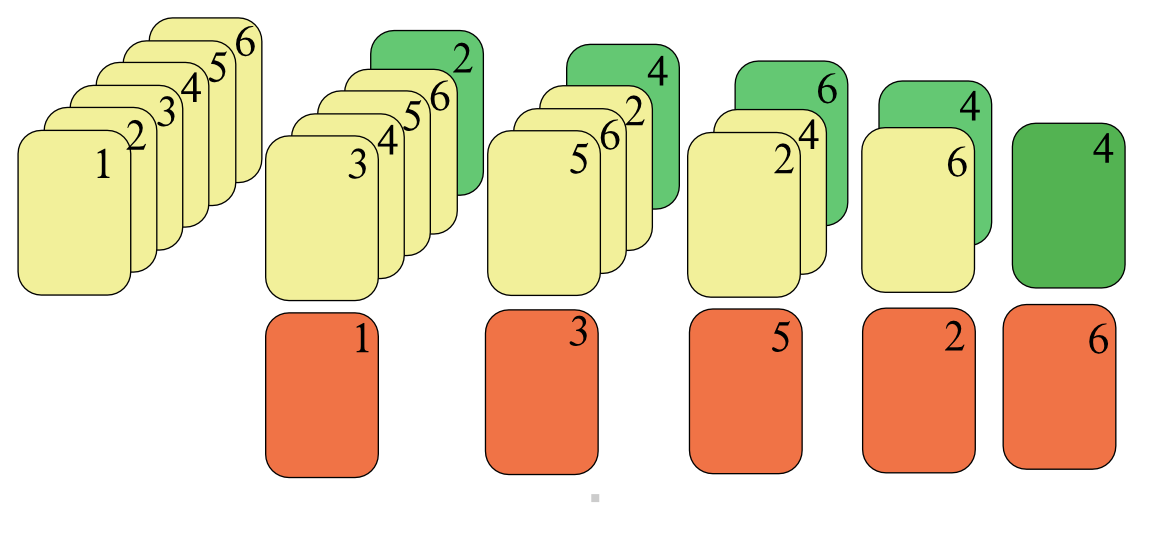
\includegraphics[width=0.9\linewidth]{throwing.png}
	\caption{Discarded cards: 1, 3, 5, 2, 6}
	\caption{Remaining card: 4}
\end{figure}
\end{frame}
%--------------------------------------------------------
\begin{frame}[fragile]
\frametitle{ Solution using queue: C++ }
\begin{example}[ C++ Implementation ]
\begin{lstlisting}
while(scanf("%d",&n), n) {
   queue <int> Q;
   for(card=1,cnt=0; card<=n; card++)
      Q.push(card);
   printf("Discarded cards:");
   while(Q.size() > 1) {
      card = Q.front(); Q.pop();
      printf("%s%d",(cnt++?", ":" "),card);
      card = Q.front(); Q.pop();
      Q.push(card);
   }
   printf("\nRemaining card: %d\n",Q.front());
}
\end{lstlisting}
\end{example}
\end{frame}
%--------------------------------------------------------
\section{Priority Queues} 
\subsection{Introduction}
\begin{frame}
\frametitle{Priority Queue}
\begin{block}{Wikipedia}
\begin{itemize}
\item In computer science, a priority queue is an abstract data type which is like a regular queue or stack data structure, but where additionally each element has a "priority" associated with it. In a priority queue, an element with high  priority is served before an element with low priority. 
\\
\item While priority queues are often implemented with heaps, they are conceptually distinct from heaps. A priority queue is an abstract concept like "a list" or "a map";
\end{itemize}
\end{block}
\end{frame}
%--------------------------------------------------------
\subsection{C++ STL Priority Queue} 

\begin{frame}
\frametitle{C++ STL Priority Queue}

\begin{block}{std::priority\_queue}
\small template $<$class T, class Container = vector$<$T$>$,\\
  class Compare = less$<$typename Container::value\_type$>>$ class priority\_queue;
\end{block}

\textbf{Priority queue}\\
Priority queues are a type of container adaptors, specifically designed such that its first element is always the greatest of the elements it contains.
\newline
\\
The container shall be accessible through random access iterators and support the following operations:

\begin{multicols}{3}
\begin{itemize}
	\item empty
	\item size
	\item front
	\item push\_back
	\item pop\_front
\end{itemize}
\end{multicols}

The standard container classes vector and deque fulfill these requirements. By default, if no container class is specified for a particular priority\_queue class instantiation, the standard container vector is used.

\end{frame}
%--------------------------------------------------------
\subsection{Challenge (Medium)}
\begin{frame}
\frametitle{Jesse and Cookies (Medium)}

\begin{block}{Description}
Jesse loves cookies. He wants the sweetness of all his cookies to be greater than value $K$. To do this, Jesse repeatedly mixes two cookies with the least sweetness. He creates a special combined cookie with:\\
\center sweetness  $=$ ($1x$Least sweet cookie $+$  $2x$ 2nd least sweet cookie).\justify
He repeats this procedure until all the cookies in his collection have a sweetness $\ge K$.\\
\textbf{You are given Jesse's cookies. Print the number of operations required to give the cookies a sweetness $\mathbf{\ge K}$. Print $\mathbf{-1}$ if this isn't possible.} 
\end{block}

\end{frame}
%--------------------------------------------------------
\subsection{Simulation \& Solution}
\begin{frame}
\frametitle{ Simulation: $N=6, K=7$ }
\begin{figure}
	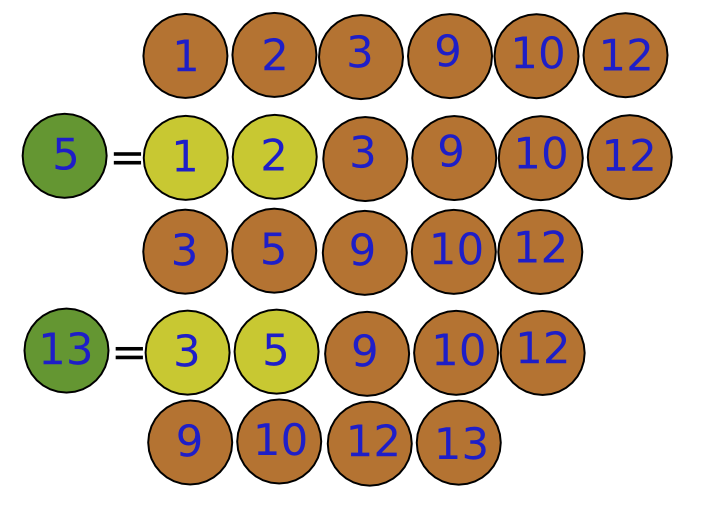
\includegraphics[width=0.5\linewidth]{cookie.png}
	\caption{Output: 2}
\end{figure}
\end{frame}
%--------------------------------------------------------
\begin{frame}[fragile]
\frametitle{ Solution using priority queue: C++ }
\begin{example}[ C++ Implementation ]
\begin{lstlisting}
   priority_queue<i64, vector<i64>, greater<i64> > PQ;
   scanf("%d %lld",&n,&k);
   for(int i=0; i<n; i++) {
      scanf("%lld",&cookie);
      PQ.push(cookie);
   }
   while(PQ.size() > 1) {
      if(PQ.top() >= k) break;
      first = PQ.top(); PQ.pop();
      second = PQ.top(); PQ.pop();
      cookie = first + second * 2LL;
      PQ.push(cookie); cnt++;
   }
   printf("%d\n",(PQ.top()<k)?-1:cnt);
\end{lstlisting}
\end{example}
\end{frame}
%--------------------------------------------------------
\subsection{Hacking Time!}
\begin{frame}[fragile]
\frametitle{ Hacking Time! }
\begin{block}{Rules}
	\begin{multicols}{2}
	\begin{itemize}
		\item 10 minutes to solve the problem.
		\item Must use priority\_queue to solve the problem.
		\item Cannot use previous solutions/implementations
		\item All test cases should pass 
	\end{itemize}
	\end{multicols}
	\textbf{short link: https://goo.gl/VyIX8N}
\end{block}
\begin{example}[ Template ]
\begin{lstlisting}
#include <queue>     // priority_queue
#include <utility>   // pair<int,int>

using namespace std; // to not use std::
typedef pair<int,int> ii; //not waste time tipping

int main() { return 0; } 
\end{lstlisting}
\end{example}

\end{frame}
%--------------------------------------------------------
\section{Double Ended Queues} 
\subsection{Introduction}
\begin{frame}
\frametitle{Double Ended Queue}
\begin{block}{Wikipedia}
\begin{itemize}
\item In computer science, a double-ended queue (dequeue, often abbreviated to deque, pronounced deck) is an abstract data type that generalizes a queue, for which elements can be added to or removed from either the front (head) or back (tail). 
\\
\item While priority queues are often implemented with heaps, they are conceptually distinct from heaps. A priority queue is an abstract concept like "a list" or "a map";
\end{itemize}
\end{block}
\end{frame}
%--------------------------------------------------------
\subsection{C++ STL Deque} 

\begin{frame}
\frametitle{C++ STL Deque}

\begin{block}{std::dueque}
template $<$ class T, class Alloc = allocator$<$T$>$ $>$ class deque;
\end{block}

\textbf{Double ended queue}\\

\textbf{deque} (usually pronounced like "deck") is an irregular acronym of double-ended queue. Double-ended queues are sequence containers with dynamic sizes that can be expanded or contracted on both ends (either its front or its back).

Specific libraries may implement deques in different ways, generally as some form of dynamic array. But in any case, they allow for the individual elements to be accessed directly through random access iterators, with storage handled automatically by expanding and contracting the container as needed.

Therefore, they provide a functionality similar to vectors, but with efficient insertion and deletion of elements also at the beginning of the sequence, and not only at its end. 

\end{frame}
%--------------------------------------------------------
\subsection{A problem solvable with Deque}
\begin{frame}
\frametitle{A problem solvable with Deque}

\begin{block}{Palindrome-Checker}
An interesting problem that can be easily solved using the deque data structure is the classic palindrome problem. A palindrome is a string that reads the same forward and backward, for example, radar, toot, and madam. We would like to construct an algorithm to input a string of characters and check whether it is a palindrome.
\newline\\
Read more in: http://goo.gl/3QVha6
\end{block}
\end{frame}
%--------------------------------------------------------
\begin{frame}
\frametitle{Palindrome-Checker}
\begin{figure}
	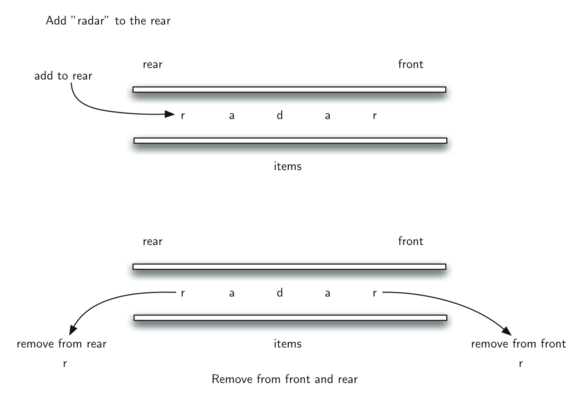
\includegraphics[width=0.85\linewidth]{palindrome.png}
	\caption{Procedure to check if a word is palindrome}
\end{figure}
\end{frame}
%--------------------------------------------------------
\subsection{Challenge (Difficult)}
\begin{frame}
\frametitle{Ocean Currents (Difficult)}

\begin{block}{Description}
At each location, the current  owes in some direction. The captain can choose to either go with the
 ow of the current, using no energy, or to move one square in any other direction, at the cost of one
energy unit. The boat always moves in one of the following eight directions: north, south, east, west,
north-east, Northwest, south-east, south-west. The boat cannot leave the boundary of the lake.\\

\textbf{You are to help him devise a strategy to reach the destination with the minimum energy consumption.}
\end{block}

\end{frame}
%--------------------------------------------------------
\begin{frame}[fragile]
\frametitle{ TO BE CONTINUE }
I left you the complete code of all previous challenges
\begin{itemize}
	\item Queue http://ideone.com/Rk7nwf
	\item Priority Q. http://ideone.com/LxR1Po
	\item Deque http://ideone.com/PvCked
	\item Session Challenge http://ideone.com/7Ldee2
\end{itemize}
\end{frame}
%--------------------------------------------------------
\begin{frame}
\frametitle{ References }
\begin{itemize}
	\item http://www.cplusplus.com/reference/queue/
	\item https://en.wikipedia.org/
\end{itemize}
\end{frame}

\end{document} 
